\subsection*{Anexo A: Formato inicial de los archivos JSON.} \addcontentsline{toc}{subsection}{Anexo A: Formato inicial de los archivos JSON.}
	\begin{figure}[H]
		\centering
		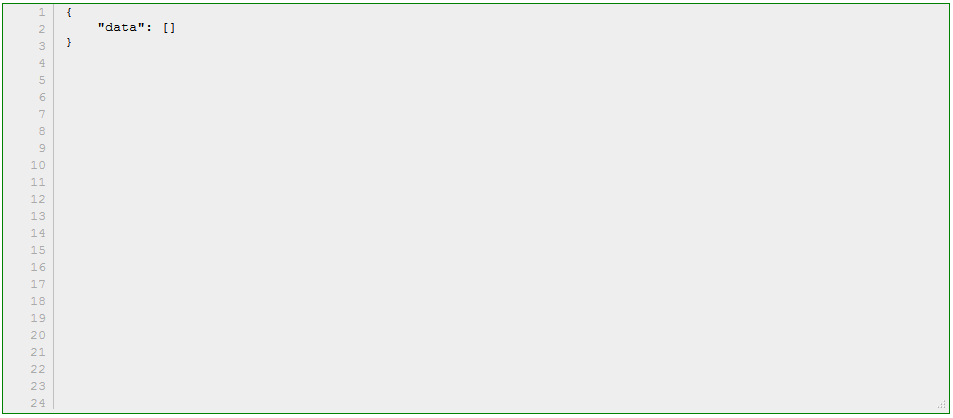
\includegraphics[width=1\textwidth]{images/Anexos/Formato_JSON.png}
		\caption[Formato inicial de los archivos JSON. ]{Formato inicial de los archivos JSON.}
		\label{Formato_json}
	\end{figure}

\subsection*{Anexo B: CascadingDropDown}\addcontentsline{toc}{subsection}{Anexo B: CascadingDropDown}

CascadingDropDown es una extención de ASP.NET AJAX que se puede conectar a un  DropDownList para obtener la población automática de un conjunto de controles DropDownList. Cada vez que se seleeciona uno de los DropDownList, el CascadingDropDown realiza una llamada a un servicio web, para recuperar la lista de valores para poblar el siguiente DropDownList.
\\

\textbf{Propiedades:}
\begin{itemize}


	\item TargetControlID: El ID de la lista desplegable a la que se aplicará.
	
	\item  Category: se define como el nombre de la categoría que la lista desplegable representa. Su utilidad será la de representar uno de los dos parámetros de entrada al ServiceMethod que estudiaremos posteriormente.
	
	\item  PromptText: Es un texto opcional que verá el usuario cuando la lista desplegable esté vacía.
	
	\item  LoadingText: Es un texto opcional que verá el usuario cuando el dato se está cargando.
	
	\item  ServicePath: Es el path del servicio web que devuelve la información que se usará para rellenar la lista desplegable.
	
	\item  ServiceMethod: Es el nombre del método el cual pobla la lista desplegable.
	
	\item  ParentControlID: ID de la lista desplegable de cuya selección depende esta lista desplegable.
	
	\item  SelectedValue: valor que vendría seleccionado por defecto. Es opcional. 
\end{itemize}



La función a la que se llamará  para rellenar la lista desplegable tendrá el siguiente formato:

 \lstset{language=C, breaklines=true, basicstyle=\footnotesize}
 \begin{lstlisting}[frame=single]
[WebMethod]

public CascadingDropDownNameValue[] GetDropDownContents(string knownCategoryValues, string category){

...
} 
 \end{lstlisting}
 
 Se puede observar que:
 \begin{itemize}
 	\item La función debe ir precedida por [WebMethod].
 	\item CascadingDropDownNameValue es un tipo de dato dentro del namespace AjaxControlToolkit.
 	\item El segundo parámetro (category)  corresponde al atributo Category que  se ha definido previamente en el control CascadingDropDown. 
 \end{itemize}
 
 
 
 \subsection*{Anexo C: Diccionario de datos.} \addcontentsline{toc}{subsection}{Anexo C: Diccionario de datos.}
 
 	\begin{figure}[H]
 		\centering
 		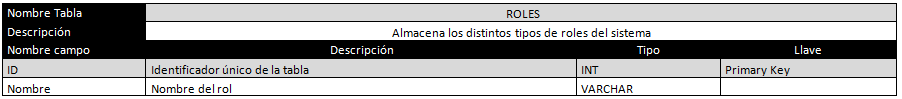
\includegraphics[width=1\textwidth]{images/Anexos/TABLA_ROLES.png}
 		\caption[Tabla ROLES ]{Tabla ROLES}
 		\label{TABLA_ROLES}
 	\end{figure}
 	
 	\begin{figure}[H]
 		\centering
 		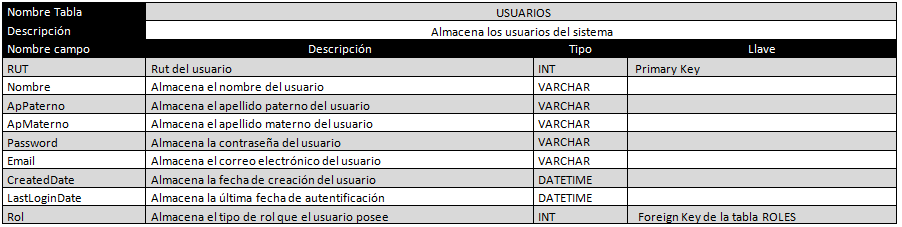
\includegraphics[width=1\textwidth]{images/Anexos/TABLA_USUARIOS.png}
 		\caption[Tabla USUARIOS ]{Tabla USUARIOS}
 		\label{TABLA_USUARIOS}
 	\end{figure}

 	\begin{figure}[H]
 		\centering
 		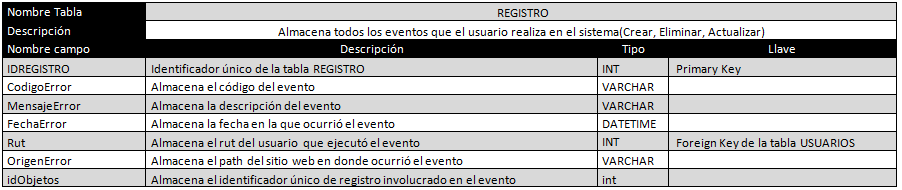
\includegraphics[width=1\textwidth]{images/Anexos/TABLA_REGISTRO.png}
 		\caption[Tabla REGISTRO ]{Tabla REGISTRO}
 		\label{TABLA_REGISTRO}
 	\end{figure}
 	
 	\begin{figure}[H]
 		\centering
 		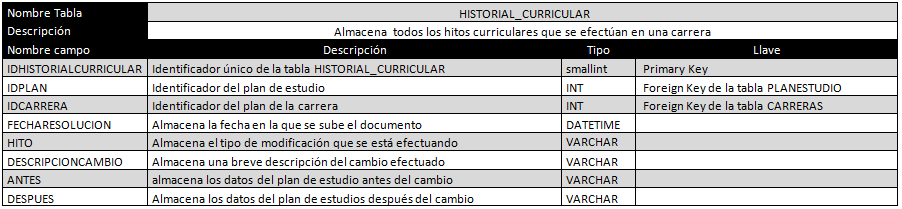
\includegraphics[width=1\textwidth]{images/Anexos/TABLA_HISTORIAL_CURRICULAR.png}
 		\caption[Tabla HISTORIAL CURRICULAR ]{Tabla HISTORIAL CURRICULAR}
 		\label{TABLA_HISTORIAL_CURRICULAR}
 	\end{figure}
 	
 	\begin{figure}[H]
 		\centering
 		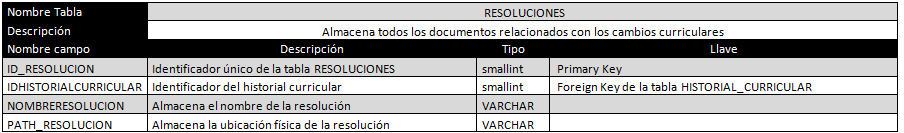
\includegraphics[width=1\textwidth]{images/Anexos/TABLA_RESOLUCIONES.png}
 		\caption[Tabla RESOLUCIONES ]{Tabla RESOLUCIONES}
 		\label{TABLA_RESOLUCIONES}
 	\end{figure}
 	
 	\begin{figure}[H]
 		\centering
 		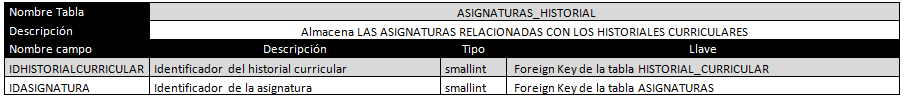
\includegraphics[width=1\textwidth]{images/Anexos/TABLA_ASIGNATURA_HISTORIAL.png}
 		\caption[Tabla ASIGNATURA HISTORIAL  ]{Tabla ASIGNATURA HISTORIAL }
 		\label{TABLA_ASIGNATURA_HISTORIAL}
 	\end{figure}